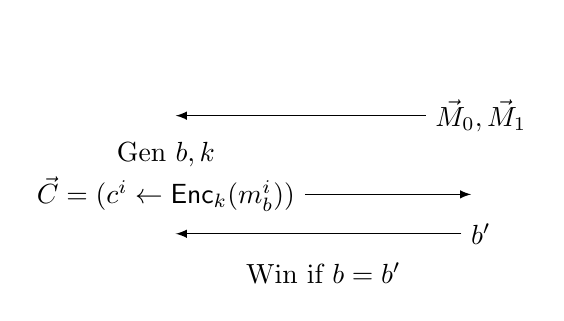
\begin{tikzpicture}
\node (A) at (0,0) {\Bob};
\node (B) [right of = A, node distance = 4cm] {\Adversary};
\node (1a) [below of=A, node distance=1cm] {};
\node (1b) [below of=B, node distance=1cm] {$\vec{M}_0, \vec{M}_1$};
\draw[-latex] (1b) -- (1a) node [midway,above] {};
\node (2a) [below of=1a, node distance=0.5cm] {Gen $b, k$};
\node (2b) [below of=1b, node distance=0.5cm] {};
%\draw[-latex] (2b) -- (2a) node [midway,above] {};
%\node (3a) [below of=2a, node distance=0.5cm] {};
%\node (3b) [below of=2b, node distance=0.5cm] {};
\node (4a) [below of=2a, node distance=0.5cm] {$\vec{C}=(c^i \gets \mathsf{Enc}_k(m_b^i))$};
\node (4b) [below of=2b, node distance=0.5cm] {};
\draw[-latex] (4a) -- (4b) node [midway,above] {};
\node (5a) [below of=4a, node distance=0.5cm] {};
\node (5b) [below of=4b, node distance=0.5cm] {$b'$};
\draw[-latex] (5b) -- (5a) node [midway,above] {};
\node (6a) [below of=5a, node distance=0.5cm] {};
\node (6b) [below of=5b, node distance=0.5cm] {};
\node (result) [right of = 6a, node distance = 2cm] {Win if $b = b'$};
\end{tikzpicture}
